\pgfplotstableset{
	begin table={\rowcolors{2}{gray!25}{white}\begin{tabular}},
	end table=\end{tabular},
}

\newcommand{\typesetfirsttable}[1]{
\noindent\begin{center}\pgfplotstabletypeset[
	skip first n=1,
	columns/10^i/.style={column name={$\varepsilon = 10^i$},},
	columns/iter/.style={column name={\scriptsize Итераций},},
	columns/fCount/.style={column name={\scriptsize Вычислений $f$},},
	columns/answer/.style={string type, column name={\scriptsize Ответ},},
	columns/restriction_value/.style={column name={$G(\mathbf{x})$},},
	columns/grad.norm()/.style={column name={$||\nabla f(x, y)||_{L_2}$}, column type/.add={}{|},},
	every head row/.style={before row=\hline,after row=\hline\hline}, 
	every last row/.style={after row=\hline},
	column type/.add={|}{},
	col sep=tab,
]{#1.txt}
\end{center}
}

\newcommand{\typesetsecondtable}[1]{
\noindent\begin{center}\pgfplotstabletypeset[
	skip first n=1,
	columns/n/.style={column name={$n$},},
	columns/iter/.style={column name={\scriptsize Итераций},},
	columns/fCount/.style={column name={\scriptsize Вычислений $f$},},
	columns/answer/.style={string type, column name={\scriptsize Ответ},},
	columns/restriction_value/.style={column name={$G(\mathbf{x})$},},
	columns/grad.norm()/.style={column name={$||\nabla f(x, y)||_{L_2}$}, column type/.add={}{|},},
	every head row/.style={before row=\hline,after row=\hline\hline}, 
	every last row/.style={after row=\hline},
	column type/.add={|}{},
	col sep=tab,
]{#1.txt}
\end{center}
}

\newcommand{\typesetfourgraphs}[1]{
\noindent\begin{tikzpicture}
\begin{semilogyaxis}[xlabel=Начальное значение штрафа,ylabel=\tcell{\scriptsize Вычислений\\\scriptsize функции},width=\textwidth, height=4cm]
\addplot[blue, no markers] table [skip first n=1, y=fCount, x=startPenaltyCoef]{table_start_#1.txt};
\end{semilogyaxis}
\end{tikzpicture}

\noindent\begin{tikzpicture}
\begin{axis}[xlabel=Начальное значение штрафа,ylabel=Итераций,width=\textwidth, height=4cm]
\addplot[red, no markers] table [skip first n=1, y=iter, x=startPenaltyCoef]{table_start_#1.txt};
\end{axis}
\end{tikzpicture}

\noindent\begin{tikzpicture}
\begin{semilogyaxis}[xlabel=Коэффициент увеличения штрафа,ylabel=\tcell{\scriptsize Вычислений\\\scriptsize функции},width=\textwidth, height=4cm]
\addplot[blue, no markers] table [skip first n=1, y=fCount, x=penaltyExponent]{table_exp_#1.txt};
\end{semilogyaxis}
\end{tikzpicture}

\noindent\begin{tikzpicture}
\begin{axis}[xlabel=Коэффициент увеличения штрафа,ylabel=Итераций,width=\textwidth, height=4cm]
\addplot[red, no markers] table [skip first n=1, y=iter, x=penaltyExponent]{table_exp_#1.txt};
\end{axis}
\end{tikzpicture}
}

%------------------------------------------------------------------------------
%------------------------------------------------------------------------------
%------------------------------------------------------------------------------

\mytitlepage{прикладной математики}{3}{Методы оптимизации}{Метод штрафных функций}{ПМ-63}{
\ltcell{Шепрут И.И.\\Крашенинник Н.А.\\Пешкичева А.А.}}{4}{Чимитова Е.В.}{2019}

\section{Цель работы}

Ознакомиться с методами штрафных функций при решении задач нелинейного программирования. Изучить типы штраф¬ных и барьерных функций, их особенности, способы и области применения, влияние штрафных функций на сходимость алгоритмов, зависимость точности решения задачи нелинейного программирования от величины коэффициента штрафа.

\section{Задание}

\noindent\begin{easylist}
\ListProperties(Hang1=true, Margin2=12pt, Style1**=$\bullet$ , Hide2=1, Hide1=1)
& Применяя методы поиска минимума 0-го порядка, реализовать программу для решения задачи нелинейного программирования с использованием метода штрафных функций/барьерных функций.
& Исследовать сходимость метода штрафных функций/барьерных функций в зависимости от:
&& выбора штрафных функций,
&& начальной величины коэффициента штрафа,
&& стратегии изменения коэффициента штрафа,
&& начальной точки,
&& задаваемой точности.
& Сформулировать выводы.
\end{easylist}

\noindent\textbf{Вариант:}

\noindent4. $f(x, y) = 2(x-y)^2+14(y-3)^2 \rightarrow min$

при ограничении:

a) $y-x \geqslant 0.2$

б) $x = -y$

\section{Исследования}

Во всех исследованиях, если не указано иное: $\varepsilon = 10^{-7}$; коэффициент увеличения штрафа: $2$; начальный коэффициент штрафа: $1$; начальное приближение: $(-1, 0)^T$; стратегия изменения штрафа: домножать текущий штраф на коэффициент увеличения штрафа.

\subsection{$y-x-0.2 \geqslant 0$}

Функция штрафа для этого случая:

$$ G = \left\{\begin{aligned}
&0, && y - x-0.2 \geqslant 0, \\
&-(y-x-0.2), && \text{иначе}
\end{aligned}\right. $$

Таблица исследования в зависимости от требуемой стартовой точности:

\typesetfirsttable{table_eps_1}

Зависимость числа вычислений функции от начальной точки. Чем темнее пиксель, тем больше требуется вычилений функции. начиная с этой точки; чем светлее, тем меньше. Границы на изображении: $[-3, 3]\times[-3, 3]$. Сверху слева показана информация о числе вычислений функции для сходимости метода из этой точки.

\noindent\begin{center}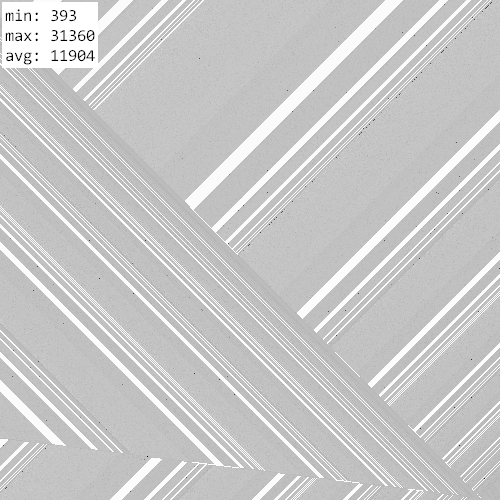
\includegraphics[width=.5\textwidth]{1.png}\end{center}

Зависимость числа итераций и вычислений функции в зависимости от начального значения штрафа и коэффициента увеличения штрафа:

\typesetfourgraphs{1}

\subsubsection{Исследования стратегии изменения штрафа}

$$ g = 100(x-y+0.2) $$

Для изменения функции штрафа была выбрана следующая функция. Будет исследовано как она влияет на процесс в зависимости от $n$:

$$ G = \left(\frac{g+|g|}{2}\right)^{2n} $$

\typesetsecondtable{table_fine_g}

\subsection{$x=-y$}

Функция штрафа для этого случая:

$$G = |x+y|$$

Таблица исследования в зависимости от требуемой стартовой точности:

\typesetfirsttable{table_eps_2}

Зависимость числа вычислений функции от начальной точки. Чем темнее пиксель, тем больше требуется вычилений функции. начиная с этой точки; чем светлее, тем меньше. Границы на изображении: $[-3, 3]\times[-3, 3]$. Сверху слева показана информация о числе вычислений функции для сходимости метода из этой точки.

\noindent\begin{center}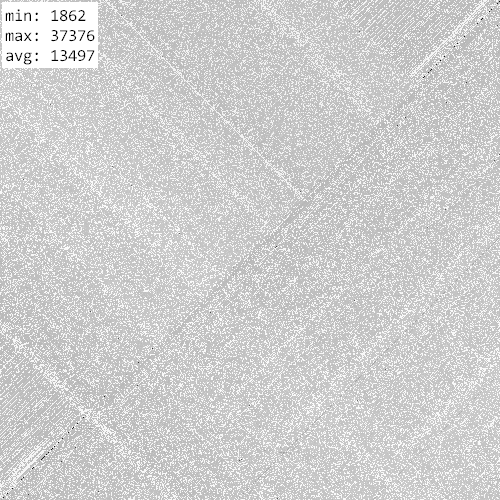
\includegraphics[width=.5\textwidth]{2.png}\end{center}

Зависимость числа итераций и вычислений функции в зависимости от начального значения штрафа и коэффициента увеличения штрафа:

\typesetfourgraphs{2}

\subsection{Барьерная функция}

Коэффициент увеличения штрафа: $0.5$ (чтобы штраф уменьшался).

$$ g = 100(x-y+0.2) $$

Функция штрафа для этого случая:

$$ G = \left\{\begin{aligned}
&-\ln(-g), && g < 0, \\
&\infty, && \text{иначе}
\end{aligned}\right. $$

Таблица исследования в зависимости от требуемой стартовой точности:

\typesetfirsttable{table_eps_3}

Зависимость числа итераций и вычислений функции в зависимости от начального значения штрафа и коэффициента увеличения штрафа:

\typesetfourgraphs{3}

\section{Выводы}

\noindent\begin{easylist}
\ListProperties(Start1=1, Hang1=true, Margin2=12pt, Style1**=, Style2**=$\bullet$ , Hide2=2, Hide1=0)
& \textit{Об объеме вычислений в зависимости от требуемой точности:}
&& Для простых штрафных функий требуемая точность практически не влияет на число вычислений.
&& Для барьерных функций требуемая точность значительно влияет на число итераций. Чем больше требуется точность, тем больше итераций.
& \textit{Об объеме вычислений в зависимости от начального приближения:} по обоим изображениям видно, что нет никакой закономерности. Хотя, возможно, потому что исследуется на квадратичной функции.
& \textit{Об объеме вычислений в зависимости от начальной величины штрафа и коэффициента изменения штрафа:} делается на основе построенных графиков
&& Для штрафных функций оптимальное начальное значение --- $10$, коэффициент увеличения штрафа --- $10$.
&& Для барьерных функций оптимальное начальное значение --- $0.1$, коэффициент увеличения штрафа --- $0.1$.
& \textit{Об объеме вычислений в зависимости от выбора штарфных функций:} функция $ G = \left(\frac{g+|g|}{2}\right)^{2n} $ практически никак не повлияла на сходимость и объем вычислений.
\end{easylist}

\section{Код}

\subsection{Заголовочные файлы}

\mycodeinput{c++}{../methods3.h}{methods3.h}
\mycodeinput{c++}{../visualize.h}{visualize.h}

\subsection{Файлы исходного кода}

\mycodeinput{c++}{../test.cpp}{make\_tables.cpp}
\mycodeinput{c++}{../methods3.cpp}{methods3.cpp}
\mycodeinput{c++}{../visualize.cpp}{visualize.cpp}